\section{~波浪模型结构与数据流} \label{chapt:run}
\newcounters

% 本章正文正按 \input 文件逐节替换为中文；表格字段和程序名需保留代码语义。
\vsssub
\subsection{~程序设计} \label{run:design}
\vssub

\ws{} 的核心是波浪模式子程序，它可由独立程序壳调用，也可由任何需要动态更新波浪数据的其他程序调用。\ws{} 发布包提供了两个这样的程序（例如 {\code ww3\_shel} 和 {\code ww3\_multi}）。辅助程序包括网格预处理器 {\code ww3\_grid}、用于生成人工初始条件的程序 {\code ww3\_strt}、用于单个 {\code ww3\_shel} 或多网格 {\code ww3\_multi} 应用的通用程序壳、两个输入预处理器（{\code ww3\_prep} 和 {\code ww3\_prnc}），以及用于网格输出数据（{\code ww3\_outf} 和 {\code ww3\_ounf}）和点输出数据（{\code ww3\_outp} 和 {\code ww3\_ounp}）的后处理器。

在本节中，文件名用 {\file file} 字体表示，文件内容用 {\code code} 字体表示，{\sc fortran} 程序元素用 {\F fortran} 字体表示。主波浪模式子程序为 {\F w3wave}。除多网格波浪模式 {\file ww3\_multi} 外，数据文件均以文件扩展名 {\file .ww3} 标识；在 {\file ww3\_multi} 中，文件扩展名标识所选多网格镶嵌中的各个网格。为简单起见，本章统一使用文件扩展名 {\file .ww3}。

包含基本数据流的关系图见图~\ref{fig:run_elements}。该图展示了一个典型工作流，如下所述。网格预处理器 {\code ww3\_grid} 写出模式定义文件 {\file mod\_def.ww3}，其中包含海底和障碍物信息，以及定义物理和数值方法的参数值。波浪模式可采用冷启动或热启动。热启动需要重启动文件 {\file restart.ww3}，该文件可由波浪模式在前一次运行中创建，也可由初始条件程序 {\code ww3\_strt} 创建。若重启动文件不可用，波浪模式将自动初始化。若打开线性增长或谱播种，模式可从平静海面（$H_s=0$）开始；否则初始条件将由基于初始风场的参数化有限风区谱组成（见初始条件程序中的相应选项）。

波浪模式例程（{\F w3wave}）可选地生成最多 9 个重启动文件 {\file restart{\em{n}}.ww3}，其中 {\file{\em{n}}} 表示一位整数。对于望远镜式嵌套应用，波浪模式还可选地从文件 {\file nest.ww3} 读取边界条件，并在 {\file nest{\em{n}}.ww3} 中为后续嵌套运行生成边界条件。此外，模式会将原始数据转储到输出文件 {\file out\_grd.ww3}、{\file out\_pnt.ww3}、{\file track\_o.ww3} 和 {\file partition.ww3}（分别为网格平均波浪参数、指定位置处的谱、沿轨迹的谱和分区波浪数据）。需输出谱的轨迹定义在文件 {\file track\_i.ww3} 中。注意，波浪模式不写标准输出，因为当 \ws{} 作为集成模式的一部分时这样会不方便。相反，它维护自己的日志文件 {\file log.ww3}，并可选地为共享内存版本输出测试文件 {\file test.ww3}，或为分布式内存版本输出 {\file test{\em{nnn}}.ww3}，其中 {\em nnn} 是从 1 开始的处理器编号。最后，还提供多种输出后处理器（原始网格场、点输出和轨迹输出文件的二进制后处理；波浪数据的 NetCDF 和 GRIB(2) 打包；用于后续 GrADS 图形处理的网格和谱数据后处理）。下文给出了所有程序元素及其输入文件的更详细说明。注意，每个例程的源代码都有完整文档。这些文档是关于 \ws{} 的额外信息来源。

\input{zh/run/fig_flow_zh}

\ws{} 专用文件在程序子例程中按名称打开。不过，单元号由用户\footnote{~{\file ww3\_multi} 除外。} 在每个 {\file \.inp} 中定义，从而保证在集成模式中实现时具有最大的灵活性。

除波浪模式子程序外，还提供初始化例程和用于数据同化的接口例程。该例程包含一个通用接口，可提供执行完整谱数据同化所需的所有模式组件。该例程集成在通用波浪模式壳中，该壳可为带或不带数据同化的波浪模式执行时间步管理。程序壳还提供一种简单而灵活的方式，将多种数据提供给数据同化方案。数据同化尚未包含在多网格波浪模式壳中。

\vssub
\subsection{~波浪模式例程} \label{sec:core}
\vssub

波浪模式驱动器是 \ws{} 框架包中的一个子程序。要运行该模式驱动子程序，需要一个程序壳。\ws{} 提供了一个简单的独立壳，见 \para\ref{sec:ww3shel}，也提供了一个更复杂的多网格模式壳，见 \para\ref{sec:ww3multi}。本节重点介绍波浪模式驱动子程序。

波浪模式初始化例程 {\F w3init} 对单个波浪模式网格执行模式初始化。这包括：通过定义单元号来建立部分 I/O 系统；初始化内部时间管理；处理模式定义文件（{\file mod\_def.ww3}）；处理初始条件（{\file restart.ww3}）；准备模式输出；以及计算依赖网格的参数。若模式为 \mpi{} 环境编译，则会确定并初始化计算和输出所需的全部通信（模式全程使用持久 \mpi{} 通信）。

在初始化完成后，可任意多次调用波浪模式例程 {\F w3wave}，以推进单个网格上的波场随时间演变。在若干初始检查之后，该子程序会插值风和流、更新冰浓度和水位、传播波场，并在若干时间步上应用所选源项。内部时间步由需要执行计算的时间区间以及请求的输出时刻共同定义。计算结束时，该例程向调用程序提供所请求的波浪数据场。{\F w3wave} 接口的文档可在源代码（{\file w3wavemd.ftn}）中找到。

\input{zh/run/fig_log_zh.tex} 

除上述原始数据文件外，程序还维护一个日志文件 {\file log.ww3}。该文件由 {\F w3init} 打开（{\F w3init} 包含在 {\file w3wavemd.ftn} 的 {\F w3wave} 中），并向该文件写入若干自解释的头部信息。对 {\F w3wave} 的每次后续调用都会在该日志文件的“动作表”中增加数行，如图~\ref{fig:log} 所示。标识为 `step' 的列显示所考虑的离散时间步。标识为 `pass' 的列给出调用 {\F w3wave} 的序列号；例如 3 表示该动作发生在第三次调用 {\F w3wave} 中。第三列显示该时间步的结束时间。输入和输出列显示模式的相应动作。{\tt X} 表示输入已更新或输出已执行。{\tt F} 表示首次读取场，{\tt L} 表示最后一次输出。七个输入列分别表示边界条件（{\tt b}）、风场（{\tt w}）、水位（{\tt l}）、流场（{\tt c}）、冰浓度（{\tt i}）以及同化数据（{\tt d}）。注意，数据同化发生在波浪例程调用之后、时间步末端。七个输出列分别表示网格输出（{\tt g}）、点输出（{\tt p}）、沿轨迹输出（{\tt t}）、重启动文件（{\tt r}）、边界数据（{\tt b}）、分区谱数据（{\tt f}）以及耦合输出（{\tt c}）。

对于多网格波浪模式 \citep[][{\file ww3\_multi}]{tol:OMOD08b}，在基本波浪模式例程周围构建了一组例程。三个主要例程是初始化例程 {\F wminit}、时间步进例程 {\F wmwave} 和终止例程 {\F wmfinl}，其功能与上述单网格例程类似。注意，原始输入和输出文件会针对镶嵌中的各个网格分别生成，并通过将标准文件扩展名 `{\file .ww3}' 替换为用户在 {\file ww3\_grid.inp} 文件中为每个单独网格选择的唯一标识符来识别。每个单独网格都维护日志文件，同时也维护一个总日志文件 {\file log.mww3}。

\vssub
\subsection{~数据同化接口} \label{sec:das}
\vssub

如上所述，波浪模式子程序还配有一个数据同化接口例程（{\file w3wdasmd.ftn} 中的 {\F w3wdas}）。该例程集成在独立壳中（见 \para\ref{sec:ww3shel}），用于为组合的波浪模式/数据同化方案提供时间步管理。它尚未集成到多网格模式驱动器中，尽管多网格模式管理算法已经考虑了它。

这里假定采用一种相当简单的方法：数据同化在选定时刻执行，而波浪模式持续向前积分。在程序壳的设置中，数据同化在模式到达目标时间之后、尚未产生输出之前执行。完成数据同化后，只为按请求生成输出而再次调用波浪模式例程。因此，给定时刻的波浪模式输出将包含该目标时刻数据同化的影响。

通用程序壳还处理若干类型的待同化数据，并将其传递给数据同化接口例程。所有数据都需要使用波浪模式输入预处理器进行预处理（见 \para\ref{sec:ww3prep}），并由通用壳通过文件名识别。目前最多可使用三个不同的数据文件。暂定而言，它们可分别为平均波浪参数、一维谱数据和二维谱数据。不过，这并未硬编码到模式中，实际上需要由用户定义。

目前尚无可用的数据同化软件包。因此，需要用户提供数据同化方案，并可使用接口例程（{\file w3wdasmd.ftn} 中的 {\F w3wdas}）将其纳入波浪模式；该例程的文档应足以支持必要的编程。关于如何将用户提供的软件添加到 \ws{} 编译系统，详见下一章。虽然 NCEP 目前正在研究波浪数据同化技术，但没有计划将波浪数据同化软件作为 \ws{} 软件包的一部分发布。

\vssub
\subsection{~辅助程序} \label{sec:auxprog}

\vsssub
\subsubsection{一般概念}
\vsssub

除轨迹输出后处理器外，这里介绍的所有辅助程序都从预定义输入文件读取输入。该文件的内容决定每个辅助程序的用户选择。注释行可用用户确定的字符表示，规则如下：输入文件第一行的第一个字符将被视为注释字符，用于在整个输入文件中标识注释行。该注释字符必须出现在输入行的第一列才有效。在以下各节的所有示例中，第一行的第一个字符为 `{\tt \$}'。因此，所有以 `{\tt \$}' 开头的行都只包含注释，不会被解析到辅助程序中。按照标准，所有辅助程序都会将格式化输出写到标准输出单元。

以下各节使用示例输入文件描述所有可用辅助程序。这些示例文件位于 \ws{} 软件包的 {\code inp} 目录中。每个示例输入文件内都包含用户可激活的全部可能选项，其中大多数以 `{\tt \$}' 开头作为注释行。本节中的文件反映示例文件的实际内容。以下各节还显示与所示输入文件相关联的可执行程序名称、程序名（如 program 语句中所示）、源代码文件，以及输入和输出文件及其单元号（在文件名后的括号中）。标有 \opt{} 的输入和输出文件为可选文件。下文提到的中间文件均为 {\F unformatted} 文件，此处不详细说明。每个文件均由单个例程写入和读取，并给出相应例程以供查阅更多文档。

\begin{list}{}{\itemsep 0mm \parsep 0mm \leftmargin 40mm \labelwidth 30mm}
\item[{mod\_def.ww3} \hfill] 子程序 {\F w3iogr}（{\file w3iogrmd.ftn}）。
\item[{out\_grd.ww3} \hfill] 子程序 {\F w3iogo}（{\file w3iogomd.ftn}）。
\item[{out\_pnt.ww3} \hfill] 子程序 {\F w3iopo}（{\file w3iopomd.ftn}）。
\item[{track\_o.ww3} \hfill] 子程序 {\F w3iotr}（{\file w3iotrmd.ftn}）。
\item[{restart.ww3}  \hfill] 子程序 {\F w3iors}（{\file w3iorsmd.ftn}）。
\item[{nest.ww3}     \hfill] 子程序 {\F w3iobc}（{\file w3iobcmd.ftn}）。
\item[{partition.ww3}\hfill] 子程序 {\F w3iosf}（{\file w3iosfmd.ftn}）。
\end{list}

\noindent
程序的预处理和编译将在后续两章讨论。源代码中提供了模式测试运行示例。

\vsssub
\subsubsection{配置文件}
\vsssub

这里介绍的所有辅助程序都从 namelist 文件（新形式）或输入文件（传统形式）读取参数和配置。虽然大多数辅助程序提供 namelist 文件选项，但仍有一些程序只能使用传统输入文件形式。后一类程序的 namelist 文件将在未来公开发布版中提供。对于已经使用 namelist 的程序，模板文件存放在 model/nml 目录中。也可以使用 model/aux/bash 目录中存放的 {\code bash} 工具，将传统 {\file inp} 文件转换为新的 {\file nml} 格式。若运行目录中同时存在 {\file inp} 和 {\file nml} 文件，则优先使用 namelist 文件。对于回归测试，默认行为是所有程序都使用 {\file inp} 文件运行；若要改用 {\file nml} 文件，必须添加 -N 选项。一些新功能仅在 namelist 中可用，未来开发也将主要面向 namelist 使用。

专用于某一程序的 namelist 配置文件提供了更易读且适应性更强的文件。一个 {\file nml} 文件包含一个或多个 namelist，每个参数都有默认值，并可由用户定义值覆盖。nml 文件中 namelist 的定义没有强制顺序。namelist 以 `{\tt \&SOMETHING\_NML}' 开始，以 `{\tt /}' 结束。若 namelist 文件跳过某一节，则会使用全部默认值。当程序读取其 namelist 文件时，所有 namelist 的默认值和用户定义值都会输出到日志文件中，以提高可追踪性。

读取程序配置的传统方式来自预定义输入文件。输入文件第一行的第一个字符将被视为注释字符，用于标识输入文件中的注释行。该注释字符必须位于输入行的第一列才有效。在以下各节的所有示例中，以 `{\tt \$}' 开头的行因此只包含注释。所有程序还会将格式化输出写到标准输出单元。

\vspace{\baselineskip} \noindent
下面给出一个 {\file inp} 文件片段及其对应的 {\file nml} 文件片段：

\vspace{\baselineskip} \noindent
\rule[1mm]{43mm}{.5mm} {\rm 示例输入文件开始（传统形式）}
\rule[1mm]{43mm}{.5mm}
\begin{footnotesize}
\begin{verbatim}
$ -------------------------------------------------------------------- $
$ WAVEWATCH III Grid preprocessor input file                           $
$ -------------------------------------------------------------------- $
$ Grid name (C*30, in quotes)
$
  'TEST GRID (GULF OF NOWHERE)   '
$
$ Frequency increment factor and first frequency (Hz) ---------------- $
$ number of frequencies (wavenumbers) and directions, relative offset
$ of first direction in terms of the directional increment [-0.5,0.5].
$ In versions 1.18 and 2.22 of the model this value was by definiton 0,
$ it is added to mitigate the GSE for a first order scheme. Note that
$ this factor is IGNORED in the print plots in ww3_outp.
$
   1.1  0.04118  32  24  0.
$
\end{verbatim}
\end{footnotesize}
\rule[1mm]{46mm}{.5mm} 示例输入文件结束（传统形式）
\rule[1mm]{45.1mm}{.5mm}

\vspace{\baselineskip} \noindent
\rule[1mm]{43mm}{.5mm} {\rm 示例输入文件开始（namelist 形式）}
\rule[1mm]{43mm}{.5mm}
\begin{footnotesize}
\begin{verbatim}
! -------------------------------------------------------------------- !
! WAVEWATCH III - ww3_grid.nml - Grid pre-processing                   !
! -------------------------------------------------------------------- !


! -------------------------------------------------------------------- !
! Define the spectrum parameterization via SPECTRUM_NML namelist
!
! * namelist must be terminated with /
! * definitions & defaults:
!     SPECTRUM%XFR   = 0.  ! frequency increment
!     SPECTRUM%FREQ1 = 0.  ! first frequency (Hz)
!     SPECTRUM%NK    = 0   ! number of frequencies (wavenumbers)
!     SPECTRUM%NTH   = 0   ! number of direction bins
!     SPECTRUM%THOFF = 0.  ! relative offset of first direction [-0.5,0.5]
! -------------------------------------------------------------------- !
&SPECTRUM_NML
  SPECTRUM%XFR           =  1.1
  SPECTRUM%FREQ1         =  0.04118
  SPECTRUM%NK            =  32
  SPECTRUM%NTH           =  24
/
\end{verbatim}
\end{footnotesize}
\rule[1mm]{46mm}{.5mm} 示例输入文件结束（namelist 形式）
\rule[1mm]{45.1mm}{.5mm}



\pb

\vsssub
\subsubsection{网格预处理器} \label{sub:ww3grid}
\vsssub

\proddefH{ww3\_grid}{w3grid}{ww3\_grid.ftn}
\proddeff{输入}{ww3\_grid.nml}{Namelist 配置文件。}{10} (App.~\ref{sec:config012})
\proddefa{ww3\_grid.inp}{传统配置文件。}{10} (App.~\ref{sec:config011})
\proddefa{'grid file' \opt}{包含海底水深的文件。}{user}
\proddefa{'obstr. file' \opt}{包含子网格障碍物的文件。}{user}
\proddefa{'mask file' \opt}{包含网格掩膜的文件。}{user}
\proddeff{输出}{standard out}{程序的格式化输出。}{6}
\proddefa{mod\_def.ww3}{\ws{} 格式的模式定义文件。}{20}
\proddefa{mask.ww3 \opt}{陆海掩膜文件（开关 {\F o2}a）。}{20}
\proddeff{暂存}{ww3\_grid.scratch}{格式化暂存文件。}{90}

\vspace{\baselineskip} \noindent
注意，海底和障碍物数据可位于同一文件中。

\pb

\vsssub
\subsubsection{初始条件程序} \label{sub:ww3strt}
\vsssub

\proddefH{ww3\_strt}{w3strt}{ww3\_strt.ftn}
\proddeff{输入}{ww3\_strt.inp}{传统配置文件。}{10} (App.~\ref{sec:config021})
\proddefa{mod\_def.ww3}{模式定义文件。}{20}
\proddeff{输出}{standard out}{程序的格式化输出。}{6}
\proddefa{restart.ww3}{\ws{} 格式的重启动文件。}{20}

\pb

\vsssub
\subsubsection{边界条件程序} \label{sub:ww3bound}
\vsssub

\proddefH{ww3\_bound}{w3bound}{ww3\_bound.ftn}
\proddeff{输入}{ww3\_bound.inp}{传统配置文件。}{10} (App.~\ref{sec:config031})
\proddefa{mod\_def.ww3}{模式定义文件。}{20}
\proddefa{'spectra file' \opt}{包含波谱的文件。}{user}
\proddeff{输出}{standard out}{程序的格式化输出。}{6}
\proddefa{nest.ww3}{边界条件文件。}{33}

\vspace{\baselineskip} \noindent
注意：当使用该程序为旋转极点网格上的模式生成边界输入时，输入谱始终假定为在标准极点上定义。

\pb

\vsssub
\subsubsection{NetCDF 边界条件程序} \label{sub:ww3bounc}
\vsssub

\proddefH{ww3\_bounc}{w3bounc}{ww3\_bounc.ftn}
\proddeff{输入}{ww3\_bounc.nml}{Namelist 配置文件。}{10} (App.~\ref{sec:config042})
\proddefa{ww3\_bounc.inp}{传统配置文件。}{10} (App.~\ref{sec:config041})
\proddefa{mod\_def.ww3}{模式定义文件。}{20}
\proddefa{'spectra file' \opt}{NetCDF 格式的波谱文件。}{user}
\proddeff{输出}{standard out}{程序的格式化输出。}{6}
\proddefa{nest.ww3}{边界条件文件。}{33}

\vspace{\baselineskip} \noindent
注意：当使用该程序为旋转极点网格上的模式生成边界输入时，输入谱始终假定为在标准极点上定义。

\pb

\vsssub
\subsubsection{输入场预处理器} \label{sec:ww3prep}
\vsssub

\proddefH{ww3\_prep}{w3prep}{ww3\_prep.ftn}
\proddeff{输入}{ww3\_prep.inp}{传统配置文件。}{10} (App.~\ref{sec:config051})
\proddefa{mod\_def.ww3}{模式定义文件。}{11}
\proddefa{'user input'\opt}{见下文示例。}{user}
\proddeff{输出}{standard out}{程序的格式化输出。}{6}
\proddefa{level.ww3\opt}{水位文件。}{12}
\proddefa{current.ww3\opt}{流场文件。}{12}
\proddefa{wind.ww3\opt}{风场文件。}{12}
\proddefa{ice.ww3\opt}{冰场文件。}{12}
\proddefa{data0.ww3\opt}{同化数据（`mean'）。}{12}
\proddefa{data1.ww3\opt}{同化数据（`1-D spectra'）。}{12}
\proddefa{data2.ww3\opt}{同化数据（`2-D spectra'）。}{12}

\vspace{\baselineskip} 
\vspace{\baselineskip} 

\noindent 
注意，可选输出文件专用于 {\file ww3\_shel} 和
{\file ww3\_multi}，但实际波浪模式例程不会处理这些文件。因此，如果波浪模式例程在其他程序壳或集成程序中使用，则不需要这些文件。不过，读写这些文件的例程与系统无关，因此可用于基本波浪模式的定制应用。这些文件的读写由子程序 {\F w3fldg}
（{\file w3fldsmd.ftn}）执行。关于更多文档和文件格式，请参考该例程。
\pb

\vsssub
\subsubsection{NetCDF 输入场预处理器} \label{sec:ww3prnc}
\vsssub

\proddefH{ww3\_prnc}{w3prnc}{ww3\_prnc.ftn}
\proddeff{输入}{ww3\_prnc.nml}{Namelist 配置文件。}{10} (App.~\ref{sec:config062})
\proddefa{ww3\_prnc.inp}{传统配置文件。}{10} (App.~\ref{sec:config061})
\proddefa{mod\_def.ww3}{模式定义文件。}{11}
\proddefa{'user input'\opt}{见下文示例。}{user}
\proddeff{输出}{standard out}{程序的格式化输出。}{6}
\proddefa{level.ww3\opt}{水位文件。}{12}
\proddefa{current.ww3\opt}{流场文件。}{12}
\proddefa{wind.ww3\opt}{风场文件。}{12}
\proddefa{ice.ww3\opt}{冰场文件。}{12}
\proddefa{data0.ww3\opt}{同化数据（`mean'）。}{12}
\proddefa{data1.ww3\opt}{同化数据（`1-D spectra'）。}{12}
\proddefa{data2.ww3\opt}{同化数据（`2-D spectra'）。}{12}

\vspace{\baselineskip} 
\vspace{\baselineskip} 
\noindent 
关于可在定制程序中用于打包输入文件的工具，见上一节（\ref{sec:ww3prep}）末尾的说明。

\pb

\vsssub
\subsubsection{潮汐预报程序} \label{sub:ww3prtide}
\vsssub

\proddefH{ww3\_prtide}{w3tide}{ww3\_prtide.ftn}
\proddeff{输入}{ww3\_prtide.inp}{传统配置文件。}{10} (App.~\ref{sec:config071})
\proddefa{mod\_def.ww3}{模式定义文件。}{20}
\proddefa{current.ww3\_tide or level.ww3\_tide}{包含潮汐分潮的文件。}{user}
\proddeff{输出}{standard out}{程序的格式化输出。}{6}
\proddefa{current.ww3 or level.ww3}{水位或流强迫。}{33}

\vspace{\baselineskip} 
\vspace{\baselineskip} 
\noindent 
用户提供的文件 current.ww3\_tide 或 level.ww3\_tide 是二进制文件，可通过使用 'AT' 选项运行 ww3\_prnc 获得，然后将所得文件 current.ww3 或 level.ww3 重命名为 current.ww3\_tide 或 level.ww3\_tide。用于潮汐预报的潮汐分潮可以是这些文件中已有分潮的一个子集，也可以是全部分潮。

由于干湿变化或网格不匹配，在某些 \ws{} 节点上，潮汐分潮可能错误或缺失。可通过对特定分量设置最大振幅来检测错误分潮。当振幅超过这些最大值时，将从最近节点外推潮汐分潮。该功能仅在三角形网格上测试过。

\pb

\vsssub
\subsubsection{通用壳程序} \label{sec:ww3shel}
\vsssub

\proddefH{ww3\_shel}{w3shel}{ww3\_shel.ftn}
\proddeff{输入}{ww3\_shel.nml}{Namelist 配置文件。}{10} (App.~\ref{sec:config082})
\proddefa{ww3\_shel.inp}{传统配置文件。}{10} (App.~\ref{sec:config081})
\proddefa{mod\_def.ww3}{模式定义文件。}{30}
\proddefa{restart.ww3}{重启动文件。}{30}
\proddefa{nest.ww3\opt}{边界条件文件。}{33}
\proddefa{level.ww3\opt}{水位文件。}{11}
\proddefa{current.ww3\opt}{流场文件。}{12}
\proddefa{wind.ww3\opt}{风场文件。}{13}
\proddefa{ice.ww3\opt}{冰场文件。}{14}
\proddefa{data0.ww3\opt}{同化数据。}{15}
\proddefa{data1.ww3\opt}{同化数据。}{16}
\proddefa{data2.ww3\opt}{同化数据。}{17}
\proddefa{track\_i.ww3\opt}{输出轨迹信息。}{22}
\proddeff{输出}{standard out}{程序的格式化输出。}{6}
\proddefa{log.ww3}{波浪模式的输出日志（见 \para\ref{sec:core}）。}{20}
\proddefa{test.ww3\opt}{波浪模式的测试输出。}{6/21}
\proddefa{restart{\sl{n}}.ww3\opt}{重启动文件。}{30}
\proddefa{nest{\sl{n}}.ww3\opt}{嵌套文件。}{34-42}
\proddefa{out\_grd.ww3\opt}{网格场原始输出。}{31}
\proddefa{out\_pnt.ww3\opt}{谱的原始输出。}{32}
\proddefa{track\_o.ww3\opt}{沿轨迹谱的原始输出。}{23}
\proddeff{暂存}{ww3\_shel.scratch}{格式化暂存文件。}{90}

\pb

\vsssub
\subsubsection{ww3\_multi 的自动网格拆分 (ww3\_gspl)} \label{sub:ww3gspl}
\vsssub

\proddefH{ww3\_gspl}{w3gspl}{ww3\_gspl.ftn}
\proddeff{输入}{ww3\_gspl.inp}{传统配置文件。}{10} (App.~\ref{sec:config091})
\proddefa{mod\_def.{\it xxx}}{待拆分网格的模式定义文件。}{11}
\proddeff{输出}{standard out}{程序的格式化输出。}{6}
\proddefa{{\it xxx}.bot}{子网格的水深文件。}{11}
\proddefa{{\it xxx}.obst}{子网格的障碍物文件。}{11}
\proddefa{{\it xxx}.mask}{子网格的掩膜文件。}{11}
\proddefa{{\it xxx}.tmpl}{子网格的 {\file ww3\_grid.inp}。}{11}
\proddefa{ww3\_multi.{\it xxx}.{\it n}}{需要修改的 {\file
ww3\_multi.inp} 部分模板。}{11}
\proddefa{ww3.ww3\_gspl}{包含子网格地图的 GrADS 文件（使用开关 {\F o16}）。}{35}
\proddefa{ww3.ctl}{GrADS 地图控制文件（{\F o16}）。}{35}

\vspace{\baselineskip} 
\noindent 
为进一步自动化网格拆分，提供了脚本 {\file ww3\_gspl.sh}。该脚本运行 {\file ww3\_gspl}，随后为所有子网格生成 {\file mod\_def} 文件。若提供了文件 {\file ww3\_multi.inp}，该文件也会被更新。脚本的工作方式可通过命令行标志 {\file -h} 显示，其输出如图~\ref{fig:gspl} 所示。

\pb

\begin{figure}[t]
{\scriptsize \input{ww3_gspl.sh.out} }
\caption{通过命令行选项 {\file -h} 运行 {\file ww3\_gspl.sh} 得到的选项说明。} \label{fig:gspl}
%\botline
\end{figure}


\clearpage

\vsssub
\subsubsection{多网格壳程序} \label{sec:ww3multi}
\vsssub

\proddefH{ww3\_multi}{w3mlti}{ww3\_multi.ftn}
\proddeff{输入}{ww3\_multi.nml}{Namelist 配置文件。}{8} (App.~\ref{sec:config102})
\proddefa{ww3\_multi.inp}{传统配置文件。}{8} (App.~\ref{sec:config101})
\proddeff{输出}{standard out}{程序的格式化输出。}{6}
\proddefa{log.mww3}{波浪模式驱动器的输出日志。}{9}
\proddefa{test.mww3\opt}{波浪模式的测试输出。}{auto}

\vspace{\baselineskip}
\noindent
该波浪模式程序需要并产生大量输入和输出文件，这些文件与 \para\ref{sec:ww3shel} 中 {\file ww3\_shel} 的文件一致；其中，文件扩展名 {\file .ww3} 会替换为特定网格的标识符。注意，所有文件均按名称打开，单元号分配是动态且自动的。

为使所有现有功能可用，现已有一个使用 namelist 的新版输入文件。这是未来将支持的版本，因为它可更灵活地添加新功能。{\bf 请注意，4.8.2 之前版本的 GCC 编译器不支持 namelist 形式。}

\pb

\vsssub
\subsubsection{网格整合} \label{sub:ww3gint}
\vsssub
\proddefH{ww3\_gint}{w3gint}{ww3\_gint.ftn}
\proddeff{输入}{ww3\_gint.inp}{传统配置文件。}{10} (App.~\ref{sec:config111})
\proddefa{mod\_def.*}{基准网格和目标网格的 \ws{} 格式模式定义文件}{20}
\proddefa{out\_grd.*}{基准网格的 \ws{} 格式网格场文件}{30+}
\proddeff{输出}{standard out}{程序的格式化输出。}{6}
\proddefa{out\_grd.*}{目标网格的 \ws{} 格式网格场文件}{30+}

\vspace{\baselineskip}
\noindent
该后处理程序从若干重叠网格获取场数据，并生成统一的输出文件。不同的模式定义文件和场输出文件由与每个特定网格关联的唯一标识符识别。目前，该程序适用于曲线网格和直角网格。程序会写出一个权重文件 {\file WHTGRIDINT.bin}；在后续使用相同源网格和目标网格的运行中可读取该文件，从而在输入网格数量较多和/或目标网格分辨率较高时节省大量时间。

\vspace{\baselineskip}
\noindent
网格整合程序可使用线性插值或最近邻插值。当分区输出用于谱重构时，建议使用后者。线性插值会导致分区扩散，从而产生虚假的能量线并人为增加总能量。
\vspace{\baselineskip}
\vspace{\baselineskip}
\noindent
注意，该程序可与网格拆分程序 {\file ww3\_gspl} 配合使用，并且 {\file ww3\_gspl.sh} 提供了为该程序生成模板输入文件的选项（见 \para\ref{sub:ww3gspl}）。

\pb

\vsssub
\subsubsection{网格输出后处理器} \label{sec:ww3outf}
\vsssub

\proddefH{ww3\_outf}{w3outf}{ww3\_outf.ftn}
\proddeff{输入}{ww3\_outf.inp}{传统配置文件。}{10} (App.~\ref{sec:config121})
\proddefa{mod\_def.ww3}{模式定义文件。}{20}
\proddefa{out\_grd.ww3}{原始网格输出数据。}{20}
\proddeff{输出}{standard out}{程序的格式化输出。}{6}
\proddefa{\ldots \opt}{传输文件。}{50}

\vspace{\baselineskip} 
\noindent
对于 {\F itype = 3}，传输文件的文件名扩展名用于标识该文件的内容。各数据类型对应的文件扩展名见第~\pageref{tab:fields} 页表~\ref{tab:fields}。

\pb

\vsssub
\subsubsection{网格输出 NetCDF 后处理器} \label{sec:ww3ounf}
\vsssub

\proddefH{ww3\_ounf}{w3ounf}{ww3\_ounf.ftn}
\proddeff{输入}{ww3\_ounf.nml}{Namelist 配置文件。}{10} (App.~\ref{sec:config132})
\proddefa{ww3\_ounf.inp}{传统配置文件。}{10} (App.~\ref{sec:config131})
\proddefa{mod\_def.ww3}{模式定义文件。}{20}
\proddefa{out\_grd.ww3}{原始网格输出数据。}{20}
\proddefa{NC\_globatt.inp}{附加全局属性（已弃用）}{994}
\proddefa{ounfmeta.inp}{用户定义的元数据属性}{60}
\proddeff{输出}{standard out}{程序的格式化输出。}{6}
\proddefa{\opt  .nc}{NetCDF 文件}{}


\vspace{\baselineskip}

\noindent
当文件中只放入一个场时，每种数据类型对应的缩写场名（来自 ww3\_outf 的文件扩展名）见第~\pageref{tab:fields} 页表~\ref{tab:fields}。

\noindent
\paragraph{元数据的用户配置：}

\noindent
默认元数据（属性）会为每个 WW3 输出变量生成到输出 netCDF 文件中。如有需要，用户可通过名为 `ounfmeta.inp' 的输入文本文件覆盖已有元数据，或配置额外元数据。


\noindent
`ounfmeta.inp' 文件可用于覆盖或配置以下内容：
\begin{itemize}
  \item 修改/扩展网格输出变量的 netCDF 属性。
  \item 修改/扩展“全局”netCDF 属性。
  \item 定义/重新定义坐标参考系统。
  \item 定义用于为分区参数输出变量生成属性的模板字符串。
\end{itemize}

\noindent
ounfmeta.inp 文件中的条目通过带有关键字标记的\emph{节}给出。空行和注释行（以 \texttt{\$} 开头）会被忽略。注意：所有关键字和 `Field Name ID' 字符串（例如 \texttt{HS}）均不区分大小写。所有 netCDF 属性名区分大小写。

\noindent
\paragraph{修改/添加 WW3 网格输出场的属性：}

\noindent
输出场通过 META 关键字选择，其后可跟整数对 \texttt{GroupNum} 和 \texttt{ParamNum}，也可跟 \texttt{FldTag} 字符串；这些值对应于 ww3\_shel.nml 或 ww3\_shel.inp 中的 `Output field parameter definitions table'。任一种形式后面都可跟一个可选整数值 \texttt{IFC}，用于在多分量场中选择分量（例如 WND 和 CUR 输出场中的 U、V 分量）。

\begin{verbatim}
  META  <GroupNum ParamNum>  |  <FldTag>  [IFC]
    attr_name  = attr_value
    attr_name  = attr_value
    extra_attr = extra_value [type]
    extra_attr = extra_value [type]
  ... repeated as many times as required.
\end{verbatim}


\noindent
每个 \texttt{attr\_name} 对应一个已有变量属性，可以是以下属性之一（括号中给出替代内部名称）：
\begin{itemize}
 \item  \texttt{standard\_name (varns)} [string]：CF 标准名称。
 \item  \texttt{long\_name (varnl)} [string]：描述性长名称。
 \item  \texttt{globwave\_name (varng)} [string]：可选 GlobWAVE 名称。
 \item  \texttt{direction\_reference} 或 \texttt{dir\_ref (varnd)} [string]：方向场的可选参考框架。
 \item  \texttt{comment (varnc)} [string]：可选注释。
 \item  \texttt{units} [string]：场的单位。
 \item  \texttt{valid\_min (vmin)} [float]：数据的最小有效值。
 \item  \texttt{valid\_max (vmax)} [float]：数据的最大有效值。
 \item  \texttt{scale\_factor (fsc)} [float]：数据缩放因子，仅当变量类型为 SHORT 时使用。
\end{itemize}

\noindent
任何其他属性名均被认为是可选的“额外”属性。该额外属性可带有可选的 `type' 关键字，用于指定元数据的变量类型。若未提供类型，则默认为字符类型。有效类型为 \texttt{[c, r, i]} 之一，分别表示字符/字符串、实数/浮点或整数值。注意：以空格分隔的字符串额外字段应加引号。

\noindent
\paragraph{修改“全局”元数据：}

\noindent
全局元数据（即与文件关联，而非与某个特定变量关联）可用特殊的 \texttt{META global} 关键字组合指定：

\begin{verbatim}
  META global [nodefault]
    extra_attr = extra_value [type]
    extra_attr = extra_value [type]
\end{verbatim}

\noindent
可选关键字 \texttt{nodefault} 会抑制默认 WW3 全局元数据的输出。

\noindent
\paragraph{修改/定义坐标参考系统：}


\noindent
可用 \texttt{CRS} 关键字为所有网格输出场指定“坐标参考系统”（CRS）。至少必须指定 \texttt{grid\_mapping\_name} 属性。若定义了 CRS 节，所有输出场都会添加一个 \texttt{grid\_mapping} 属性，引用 CRS 变量。\texttt{crs\_vaname} 将在输出文件中创建为一个标量 NF90\_CHAR 变量。

\begin{verbatim}
  CRS <crs_varname>
    grid_mapping_name = <mapping name>
    attr = value
    attr = value
\end{verbatim}

\noindent
对于普通经纬度网格和旋转极点网格，ww3\_ounf 会生成合适的坐标参考系统，但可使用 CRS 关键字覆盖。


\noindent
\paragraph{分区参数模板字符串}

\noindent
分区输出的元数据指定方式略有不同；一个元数据条目用于某一场的所有分区。元数据通过\emph{模板字符串}针对特定分区编号专门化。内置模板字符串有两个：\texttt{SPART} 和 \texttt{IPART}。它们分别提供“字符串”描述（例如 `wind sea'、`primary swell' 等）或整数分区编号（1、2、3 等）。可在元数据属性值中用被 \texttt{< ... >} 包围的模板名引用它们，例如 \texttt{<SPART>}。

\noindent
也可以在 ounfmeta.inp 文件中用 \texttt{TEMPLATE} 关键字提供用户定义的分区参数模板字符串，如下所示：

\begin{verbatim}
  TEMPLATE <template-name>
    String for partition 0
    String for partition 1
    String for partition 2
    String for partition 3
    ... etc
\end{verbatim}

\noindent
若指定带有尾随下划线的 \texttt{<template-name>}，则会提供以下划线分隔（\texttt{\_}）而不是以空格分隔的字符串（这对 netCDF `standard name' 值很有用）。


\noindent
\paragraph{ounfmeta.inp 文件示例：}
\begin{verbatim}
   $ Lines starting with dollars are comments.
   $ The line starts a meta-data section for the depth field
   META DPT
     standard_name = depth
     long_name = "can be quoted string"
     comment = or an unquoted string
     vmax = 999.9

   $ Next one is HSig (group 2, field 1)
   META 2 1
     varns = "sig. wave height"
     varnl = "this is long name"

   $ Next one is second component of wind. It also sets an
   $ "extra" meta data value (height - a float)
   META WND 2
     standard_name = "v-wind"
     height = 10.0 "r"

   $ User defined partitioned parameters template strings:
   TEMPLATE PARTSTR
     wind wave
     primary swell
     secondary swell

   $ Use partition templates in partitioned Hs field:
   $ (SPART and IPART are built-in)
   META PHS
     standard_name = "<SPART_>_sigificant_wave_height"
     long_name = "<PARTSTR>"
     partition_number = "<IPART>"

   $ Coordinate reference system:
   CRS crs
     grid_mapping_name = "latitude_longitude"
     semi_major_axis = 6371000.0 f
     inverse_flattening = 0 f

   $ Global metadata:
   META global
     institution = UKMO
     comment "space seperated strings should be quoted" c
     version = 1.0 r

\end{verbatim}


\noindent
\paragraph{添加“forecast variables”：}
使用 ww3\_ounf.nml 输入文件时，可向输出 netCDF 文件添加可选辅助“forecast variables”（见 ww3\_ounf.nml）。当 \texttt{FCVARS = T} 时，将生成以下变量：
\begin{itemize}
 \item \texttt{forecast\_reference\_time}：与当前预报的“分析”关联的时间。对于跨多天拆分的文件很有用，因为它允许把某一特定时刻的预报追溯到其分析时间或起始时间。
 
 \item \texttt{forecast\_period}：自关联的 \texttt{forecast\_reference\_time} 起经过的时间段（单位为秒）。
\end{itemize}

\noindent
\texttt{forecast\_reference\_time} 默认为 ww3\_ounf.nml 中指定的 \texttt{TIMESTART}。不过，模式运行可能包含某种后报时段；在这种情况下，\texttt{forecast\_reference\_time} 应设置为合适的分析时间。此外，如果调用 ww3\_ounf 时使用的 \texttt{TIMESTART} 与模式起始时间不同，则需要显式指定正确的 \texttt{forecast\_reference\_time}，以确保 \texttt{forecast\_period} 计算正确。

\pb

\vsssub
\subsubsection{用于 GrADS 的网格输出后处理器} \label{sec:gxoutf}
\vsssub

\proddefH{gx\_outf}{gxoutf}{gx\_outf.ftn}
\proddeff{输入}{gx\_outf.inp}{传统配置文件。}{10} (App.~\ref{sec:config141})
\proddefa{mod\_def.ww3}{模式定义文件。}{20}
\proddefa{out\_grd.ww3}{原始网格输出数据。}{20}
\proddeff{输出}{standard out}{程序的格式化输出。}{6}
\proddefa{ww3.grads}{GrADS 数据文件。}{50}
\proddefa{ww3.ctl}{GrADS 控制文件。}{51}

\vspace{\baselineskip} 
\noindent 
该后处理器为 Grid Analysis and Display System \citep[GrADS,][]{man:GrADS} 生成包含网格模式参数的输入文件。
%This graphical software can be obtained from http://www.iges.org/grads.  -- website no longer valid
虽然 GrADS 也可处理 GRIB 文件，但当前预处理器更合适，因为该数据文件还可访问陆-海-冰地图。

\pb

\vsssub
\subsubsection{网格 GRIB 输出后处理器} \label{sec:ww3grib}
\vsssub

\proddefH{ww3\_grib}{w3grib}{ww3\_grib.ftn}
\proddeff{输入}{ww3\_grib.inp}{传统配置文件。}{10} (App.~\ref{sec:config151})
\proddefa{mod\_def.ww3}{模式定义文件。}{20}
\proddefa{out\_grd.ww3}{原始网格输出数据。}{20}
\proddeff{输出}{standard out}{程序的格式化输出。}{6}
\proddefa{gribfile}{GRIB 文件。}{50}

\vspace{\baselineskip} 
\noindent
该后处理器将平均波浪参数场打包为 GRIB 格式，可使用 GRIB version II 和 \ncep{} 的 w3 与 bacio 库例程，或使用 GRIB2 及 NCEP 的业务软件包。附加打包数据见第~\pageref{tab:fields} 页表~\ref{tab:fields}。

GRIB 打包使用 \ncep{} 的 GRIB 表，见 \cite{rep:GRIB1}。由于 w3 和 bacio 例程并非完全可移植，它们不随代码提供。用户必须提供相应例程。建议使用强制开关组中包含 `{\F nogrb}' 开关的附加 \ws{} 开关来激活这些例程，就像目前 \ncep{} 例程的情况一样。GRIB2 打包按照 \cite{rep:GRIB2} 执行，并使用 NCEP 的标准业务软件包。

表~\ref{tab:fields} 显示用于 GRIB 打包的 {\F kpds(5)} 数据值。对于分区数据，第一个数字表示风海，第二个数字表示涌浪。多数数据作为表面数据打包（{\F
kpds(6) = 0}）。不过，对于分区涌浪场，连续场会按连续层打包，层类型指示符设为（{\F
kpds(6) = 241}）。{\F kpds(7)} 标识实际层或涌浪场编号。

表~\ref{tab:fields} 还显示若干用于 GRIB2 打包的 {\F kpds} 数据值。表中第一个数字表示 {\F listsec0(2)}，用于标识 discipline 类型（例如海洋学、气象学等）。第二个数字表示 {\F kpds(1)}，用于标识该 discipline 类型内的参数类别（例如波浪、环流、海冰等）。第三个数字表示 {\F kpds(2)}，用于标识实际参数。对于分区数据，A/B 表示 A 用于风海、B 用于涌浪。此外，{\F kpds(10) = 0} 用于表面数据，{\F kpds(10) = 241 } 用于在连续层上打包连续涌浪场。{\F kpds(12)} 标识实际层或涌浪场编号。

尽管上述输入文件包含 \ws{} 全部 31 个输出场的标志，但并非所有场都可打包为 GRIB。如果选择了没有 GRIB 打包支持的参数，程序会向标准输出打印消息。表~\ref{tab:fields} 显示哪些参数可打包为 GRIB。注意，在 \ncep{}，从 GRIB 到 GRIB2 的转换与分区波浪模式输出的引入同时发生。这导致 GRIB 中出现一些重复定义，并导致 GRIB 和 GRIB2 打包之间出现一些表面上的不一致。

\pb

\vsssub
\subsubsection{点输出后处理器} \label{sec:ww3outp}
\vsssub

\proddefH{ww3\_outp}{w3outp}{ww3\_outp.ftn}
\proddeff{输入}{ww3\_outp.inp}{传统配置文件。}{10} (App.~\ref{sec:config161})
\proddefa{mod\_def.ww3}{模式定义文件。}{20}
\proddefa{out\_pnt.ww3}{原始点输出数据。}{20}
\proddefa{NC\_globatt.inp}{附加全局属性。}{994}
\proddeff{输出}{standard out}{程序的格式化输出。}{6}
\proddefa{tab{\sl{nn}}.ww3 \opt}{平均参数表，其中
{\file{\sl{nn}}} 为两位整数。}{\sl nn}
\proddefa{\ldots \opt}{传输文件。}{user}

\vspace{\baselineskip} 
\vspace{\baselineskip} 
\noindent 
在 \ws{} 早期版本中，谱公报使用由 {\F itype = 1} 和 {\F otype = 3} 生成的谱数据传输文件以及 {\file w3split} 程序（见 section~\ref{sec:install}）生成。这是一段即将淘汰的代码，此处仅为向后兼容而提供。该程序从标准输入读取以下五条记录（不允许注释行）：

\begin{list}{$\bullet$}{\itemsep 0mm \parsep 0mm}
\item 输出位置名称。
\item 表中使用的运行标识符。
\item 输入文件名称。
\item 标识 UNFORMATTED 输入文件的逻辑量。
\item 输出文件名称。
\end{list}

\noindent
以上所有字符串均以自由格式按字符读取，因此需要用引号括起。

\pb

\vsssub
\subsubsection{点输出 NetCDF 后处理器} \label{sec:ww3ounp}
\vsssub

\proddefH{ww3\_ounp}{w3ounp}{ww3\_ounp.ftn}
\proddeff{输入}{ww3\_ounp.nml}{Namelist 配置文件。}{10} (App.~\ref{sec:config172})
\proddefa{ww3\_ounp.inp}{传统配置文件。}{10} (App.~\ref{sec:config171})
\proddefa{mod\_def.ww3}{模式定义文件。}{20}
\proddefa{out\_pnt.ww3}{原始点输出数据。}{20}
\proddeff{输出}{standard out}{程序的格式化输出。}{6}
\proddefa{\ldots \opt}{传输文件。}{user}

\vspace{\baselineskip} 
\noindent 

\pb

\vsssub
\subsubsection{用于 GrADS 的点输出后处理器} \label{sec:gxoutp}
\vsssub

\proddefH{gx\_outp}{gxoutp}{gx\_outp.ftn}
\proddeff{输入}{gx\_outp.inp}{传统配置文件。}{10} (App.~\ref{sec:config181})
\proddefa{mod\_def.ww3}{模式定义文件。}{20}
\proddefa{out\_pnt.ww3}{原始点输出数据。}{20}
\proddeff{输出}{standard out}{程序的格式化输出。}{6}
\proddefa{ww3.spec.grads}{包含谱和源项的 GrADS 数据文件。}{30}
\proddefa{ww3.mean.grads}{包含平均波浪参数的文件。}{31}
\proddefa{ww3.spec.ctl}{GrADS 控制文件。}{32}

\vspace{\baselineskip} 
\noindent
该后处理器用于生成数据文件，使 GrADS（见上一节）能够绘制谱和源项的极坐标图。为实现这一点，谱和源项被存储为“经度-纬度”网格。对于每个输出点，会为数据生成不同名称，通常为 {\F
loc{\it nnn}}。当数据文件载入 GrADS 时，变量 {\F loc001} 将在第 1 层包含第一个请求输出点的谱网格，在第 2 层包含输入源项，依此类推。对于第二个输出点，数据存储在 {\F loc002} 中，依此类推。实际输出点名称通过控制文件 {\file ww3.spec.ctl} 传递给 GrADS。波高和环境数据从 {\file ww3.mean.grads} 获取。不过，用户无需了解 GrADS 数据文件和数据存储的细节。程序提供了 GrADS 脚本 {\file spec.gs}、{\file source.gs} 和 {\file 1source.gs}，用于从该后处理器的输出文件自动生成谱图。

注意：为使 GrADS 脚本正常工作，输出点名称不应包含空格。

\pb

\vsssub
\subsubsection{轨迹输出后处理器} \label{sec:ww3trck}
\vsssub

\proddefH{ww3\_trck}{w3trck}{ww3\_trck.ftn}
\proddeff{输入}{ww3\_trck.inp}{传统配置文件。}{10} (App.~\ref{sec:config191})
\proddefa{track\_o.ww3}{原始轨迹输出数据。}{11}
\proddeff{输出}{standard out}{程序的格式化输出。}{6}
\proddefa{track.ww3}{格式化数据文件。}{51}

\vspace{\baselineskip}
\noindent
该后处理器将原始轨迹输出数据转换为整数压缩的格式化文件。该文件包含以下头记录：

\begin{list}{$\bullet$}{\itemsep 0mm \parsep 0mm}
\item 文件标识符（长度为 34 的字符串）。
\item 频率数和方向数、第一个方向以及方向增量（弧度，海洋学约定）。
\item 每个频率箱的弧频率。
\item 对应的方向箱宽乘以频率箱宽，用于得到每个离散箱的能量。
\end{list}

\noindent
对于随时间和位置变化的每个输出点，将写出以下记录：
\begin{list}{$\bullet$}{\itemsep 0mm \parsep 0mm}
\item {\tt yyyymmdd hhmmss} 格式的日期和时间、以度为单位的经度和纬度，以及状态标识符
      `{\F ice}'、`{\F lnd}' 或 `{\F sea}'。以下两条记录仅对海点写出。
\item 以米为单位的水深，以米每秒为单位的海流和风的 $u$、$v$ 分量，
      以米每秒为单位的摩擦速度，以摄氏度为单位的气海温差，以及谱的缩放因子。
\item 以整数打包格式给出的完整谱（可用自由格式读取）。
\end{list}

\pb

\vsssub
\subsubsection{轨迹输出 NetCDF 后处理器} \label{sec:ww3trnc}
\vsssub

\proddefH{ww3\_trnc}{w3trnc}{ww3\_trnc.ftn}
\proddeff{输入}{ww3\_trnc.nml}{Namelist 配置文件。}{10} (App.~\ref{sec:config202})
\proddefa{ww3\_trnc.inp}{传统配置文件。}{10} (App.~\ref{sec:config201})
\proddefa{track\_o.ww3}{原始轨迹输出数据。}{11}
\proddeff{输出}{standard out}{程序的格式化输出。}{6}
\proddefa{*.nc}{NetCDF 文件。}{}

\vspace{\baselineskip}
\noindent
该后处理器将原始轨迹输出数据转换为 NetCDF 文件。输出 NetCDF 文件包含以下变量：

\begin{list}{$\bullet$}{\itemsep 0mm \parsep 0mm}
\item 自 1990-01-01 起算的天数形式的时间，即 UTC 时间下的儒略日。
\item 每个频率箱的频率（弧度）。
\item 每个频率箱下边带的频率（弧度）。
\item 每个频率箱上边带的频率（弧度）。
\item 每个频率箱的频率宽度（弧度）。
\item 每个方向箱的方向（海洋学约定）。
\item 沿时间维度给出的纬度和经度（度）。
\end{list}

\noindent
对于随时间和位置变化的每个输出点，将写出以下记录：
\begin{list}{$\bullet$}{\itemsep 0mm \parsep 0mm}
\item 轨迹名称（32 个字符）。
\item 完整谱（m2 s rad-1）。
\item 水深（m），海流和风的 $u$、$v$ 分量（m s-1），摩擦速度（m s-1），气海温差（摄氏度）。
\end{list}

\pb

\vsssub
\subsubsection{波浪系统的时空跟踪} \label{sec:ww3systrk}
\vsssub

\proddefH{ww3\_systrk}{w3systrk}{ww3\_systrk.ftn}
\proddeff{输入}{ww3\_systrk.inp}{传统配置文件。}{10} (App.~\ref{sec:config211})
\proddefa{partition.ww3}{谱分区文件。}{11}
\proddefa{sys\_restart.ww3\opt}{带系统记忆的重启动文件。}{12}
\proddefa{sys\_mask.ww3\opt}{掩膜文件。}{13}
\proddeff{输出}{sys\_log.ww3}{输出日志（并行运行时附加处理器编号）。}{20}
\proddefa{sys\_coord.ww3}{场的经纬度坐标。}{21}
\proddefa{sys\_hs.ww3}{各个波浪系统的有效波高场。}{22}
\proddefa{sys\_tp.ww3}{各个波浪系统的峰值周期场。}{23}
\proddefa{sys\_dir.ww3}{各个波浪系统的峰值方向场。}{24}
\proddefa{sys\_dspr.ww3}{各个波浪系统的方向扩展场。}{25}
\proddefa{sys\_pnt.ww3}{有效波高、峰值周期和峰值方向的点输出文件。}{26}
\proddefa{sys\_restart1.ww3}{重启动文件。}{27}
\proddefa{*.nc}{NetCDF 文件。}{ }

\vspace{\baselineskip}
\noindent
该程序目前仅实现于规则网格。时空跟踪基于谱分区数据文件进行。用于跟踪波浪系统的时间区间和地理区域都可以是分区文件所含数据的子集。组合参数 {\code dirKnob} 和 {\code perKnob} 用于影响地理空间中系统组合算法的严格程度，{\code dirTimeKnob} 和 {\code perTimeKnob} 则是在时间空间中的对应参数。较低的数值意味着更严格的判据，从而得到更小、数量更多的系统；这通常也会增加处理时间。上文给出了推荐值。这些值可以通过定义掩膜文件 {\file sys\_mask.ww3} 在局地进行调整，例如在岛屿周围。参数 {\code hsKnob} 和 {\code wetPts} 是低能量与小系统过滤器，即所有平均 $H_\mathrm{m0}$ 低于 {\code hsKnob} 的波浪系统，或尺寸小于整个区域大小的 {\code wetPts}*100\% 的波浪系统，都会被剔除。参数 {\code seedLat} 和 {\code seedLon} 影响波浪系统搜索螺旋的起点；默认值位于模式区域中心（由 {\code 0. 0.} 表示）。跟踪运行结束时，系统记忆的结束状态存储在 {\file sys\_restart1.ww3} 中。将该文件改名为 {\file sys\_restart.ww3} 后，可用于从先前的系统记忆状态重启动跟踪序列。

\pb

\vsssub
\subsubsection{重启动文件处理器} \label{sec:ww3uprstr}
\vsssub

\proddefH{ww3\_uprstr}{ww3uprstr}{ww3\_uprstr.ftn}
\proddeff{输入}{ww3\_uprstr.inp}{传统配置文件。}{10} (App.~\ref{sec:config221})
\proddefa{mod\_def.ww3}{模式定义文件。}{20}
\proddefa{restart.ww3}{重启动文件。}{ }
\proddefa{XXXX.grbtxt}{grbtxt 格式的有效波高分析文件。}{123}
\proddeff{输出}{restart001.ww3}{更新后的重启动文件。}{ }

\vspace{\baselineskip}

\paragraph{引言 \newline}

海面波浪场的大多数观测都是诊断变量有效波高（SWH）的观测。因此，波浪资料同化（WDA）常常在 SWH 空间中进行，随后需要把这些信息转换到预报变量空间，也就是波谱（WS），以便作为边界和/或初始条件（BIC）施加。

\subparagraph{\textbf{ww3\_uprstr} 的目的 \newline}
将 SWH 场分析中的能量重新分配到保存在重启动文件中的 WS 场。

\subparagraph{核心算法 \newline}
\textbf{ww3\_uprstr} 将背景谱的 SWH 设置为等于分析 SWH，并根据用户指定的谱形修改谱的形状。\textbf{ww3\_uprstr} 作为重启动读取器的扩展实现；它需要的输入包括重启动文件、分析 SWH，以及包含用户定义选项的 \textbf{ww3\_uprstr.inp}（见上文）。为减少即时计算，可能还需要额外文件。

\paragraph{如何使用 ww3\_uprstr \newline}
使用 \textbf{ww3\_uprstr} 时，用户需要遵循与所有 WAVEWATCH III 程序相同的逻辑。概括如下：

\begin{enumerate}
   \item \textbf{下载源代码} \newline
   从 6.07 版开始，\textbf{ww3\_uprstr} 源代码已经包含在 WAVEWATCH III 官方发布版中。
   \item \textbf{编译代码} \newline
   \textbf{ww3\_uprstr} 的编译方式与 WAVEWATCH III 的其他辅助程序相同，见手册中的相应章节。若需要调试输出，在 switch 文件中使用 \textbf{T} 标志。
   \item \textbf{测试可执行程序} \newline
   回归测试 \textbf{ww3\_ta1} 可用于测试 \textbf{ww3\_uprstr} 的不同选项。
   \item \textbf{运行 ww3\_uprstr} \newline
   运行 \textbf{ww3\_uprstr} 的步骤说明：
   \begin {description}
      \item{必需输入文件：\newline}
      \begin{itemize}
         \item \textbf{重启动文件。} 该文件由 WW3 在模式后报运行或前一循环中创建。预期文件名为 \textbf{restart.ww3}。
         \item \textbf{mod\_def.ww3}
         \item \textbf{ww3\_uprstr.inp。} 这是 \textbf{ww3\_uprstr} 的输入文件。用户必须定义：i. 同化日期；ii. 能量重新分配方法；iii. 取决于所选方法的百分比或输入文件。
         \item \textbf{分析输入文件。} 文件可以使用任意名称，但后缀决定用于导入数据的读取器。对大多数选项，读取器仅支持 \textbf{grbtxt} 格式。这是一个由 wgrib2 从分析 grib2 文件创建的文本文件，其结构如下：\newline

         \begin{tabular}{|c|}
            \hline
            NX NY       \\
            VAL0001     \\
            VAL0002     \\
            ...         \\
            VAL(NX*NY)  \\
            \hline
          \end{tabular}
    \newline
    \item 运行可执行程序：\newline
          \textgreater \$EXE/ww3\_uprstr \newline
          如果所有输入都准备正确，将创建新的重启动文件（\textbf{restart001.ww3}）。\textbf{ww3\_uprstr} 按与 restart.ww3 相同的格式导出更新后的谱。若要把它作为下一预报循环初始化的 BIC 使用，必须将其改名：\newline
          \textgreater mv \textbf{restart001.ww3} \textbf{restart.ww3}) \newline
          更新后的重启动文件随后即可按常规方式使用。
      \end{itemize}
   \end{description}

   \noindent\fbox{
      \parbox{\textwidth}{
         \textbf{提示}
         \begin{itemize}
            \item 重启动文件必须使用与 \textbf{ww3\_uprstr} 相同的 WW3 版本创建；该工具不提供向后兼容性。
            \item 在 \textbf{ww3\_uprstr.inp} 中定义的同化开始时间必须与重启动文件中的时间一致。
            \item 使用 \textbf{T} 时，\textbf{ww3\_uprstr.inp} 会导出背景重启动文件、分析以及更新后重启动文件中的 SWH 场。此外，更新前后的重启动文件谱也会作为文本文件导出。
         \end{itemize}
         }
   }
\end{enumerate}

\subparagraph{更新方法 \newline}
用户必须在 \textbf{ww3\_uprstr.inp} 中定义自己选择的更新算法。更新重启动文件的选项通过标志 UPD[N] 在 ww3\_uprstr.inp 中定义，其中 N 可以为 0F、0C、1、2 等。对于 N \textless 2 的 UPDN，同一修正应用于整个网格；预期输入为 PRCNTG，如 fac 所定义。对于 N \textgreater 1 的 UPDN，每个网格点都有自己的更新因子，输入为 grb2txt 格式。当前实现的更多细节见图~\ref{fig:uprstrflowchart}。

\begin{figure} \begin{center}
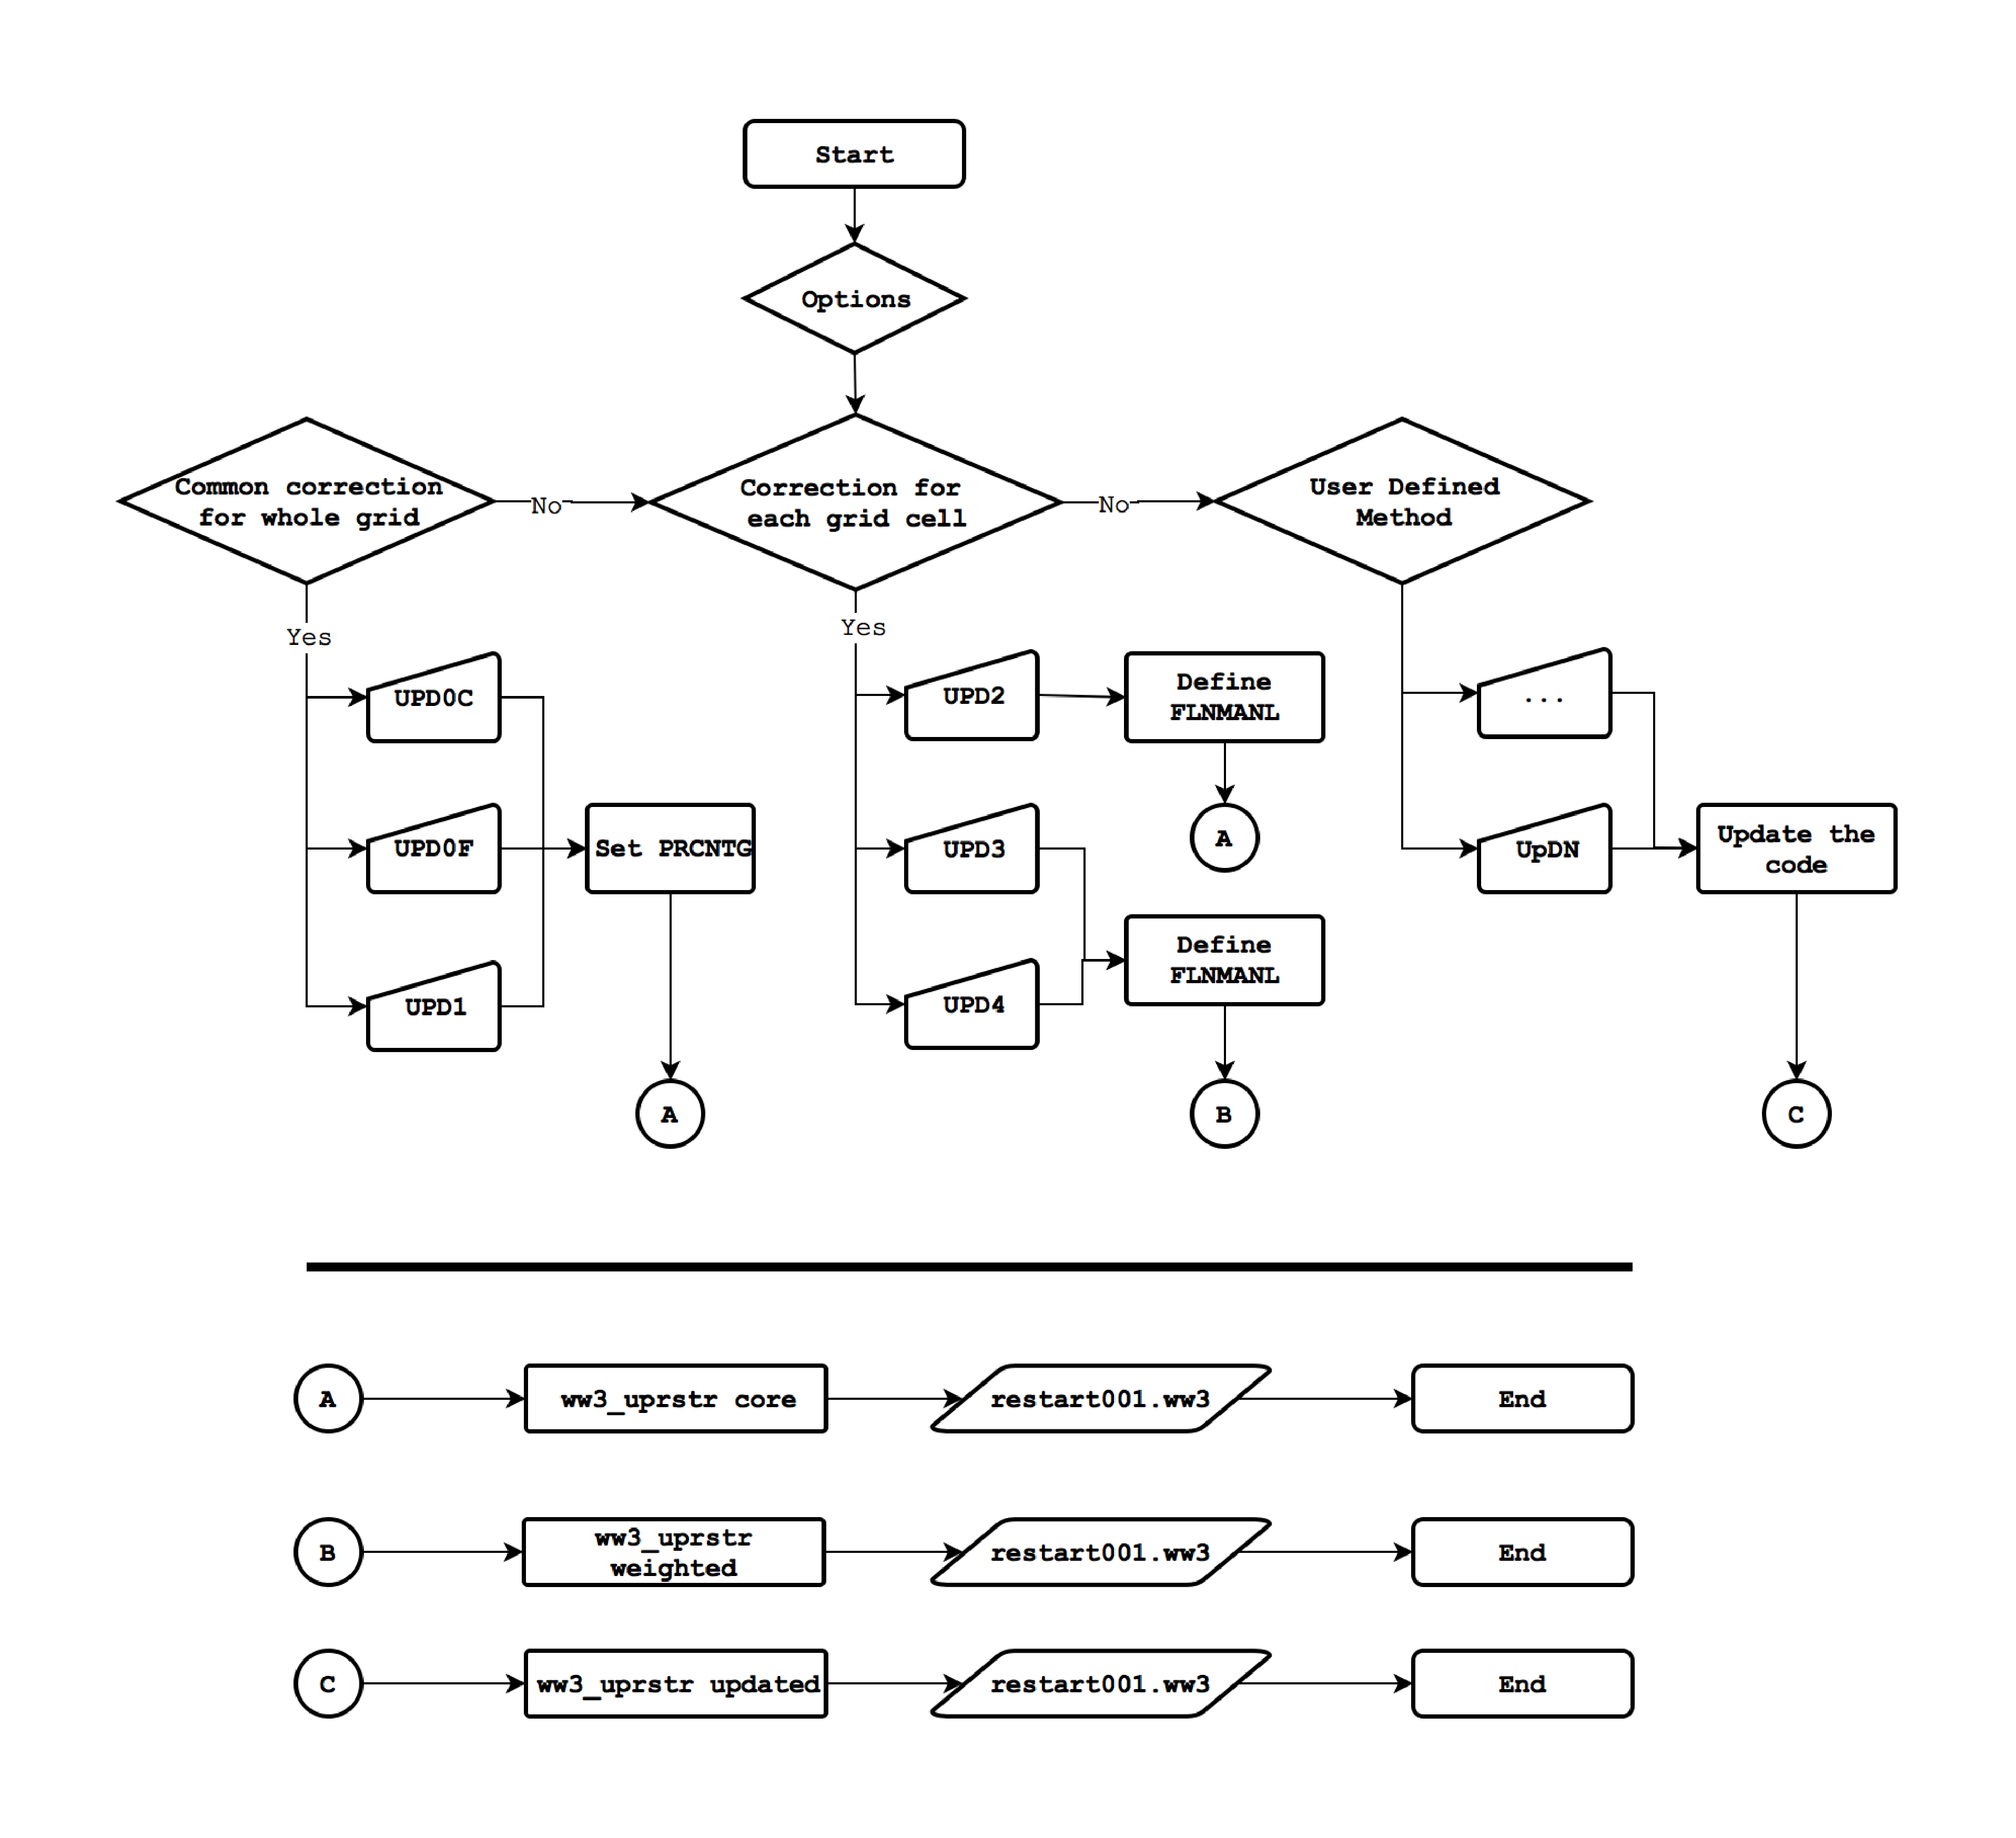
\includegraphics[width=0.9\textwidth]{./run/uprstr.eps}
\caption{WW3 重启动文件中波谱更新方法的实现流程图。可通过在 namelist 中增加 UPD 选项来实现其他方法。}
\label{fig:uprstrflowchart} \botline
\end{center}
\end{figure}

目前可用的 UPD 选项如下：
\begin{enumerate}
   \item UPD0C:: \textbf{自 5.16 版起已删除} 选项 0C，所有谱使用一个常数更新：\newline
      \(fac=(SWH\_Bckg-SWH\_Anl)/SWH\_Anl \).
   \item UPD0F:: 选项 0F，所有谱使用一个常数更新：\newline
      \(fac=SWH\_Anl/SWH\_Bckg \).
   \item UPD1 :: \textbf{自 5.16 版起已删除} 选项 1，fac(x,y,frq,theta) 按每个谱箱中的能量百分比加权；fac 与 UPDOF 相同。
   \item UPD2 :: 选项 2，根据 SWH\_Bckg 和 SWH\_Anl 在每个网格点计算 fac(x,y,frq,theta)。
   \item UPD3 :: 选项 3，更新因子是一个具有背景谱形状的曲面。
   \item UPD4 :: [当前版本未包含，仅保留位置] 选项 4，UPD3 的一般化。更新因子为多个曲面的和，这些曲面施加到背景谱上。该算法需要将每个分区映射到单个谱；该映射用于确定加权曲面。
   \item UPD5 :: 选项 5，修正按 UPD2 计算，但仅当风海为主导分量时才应用于谱的风海部分；否则修正整个谱。必需输入为分析 Hs 场，以及背景风速和风向。若要包含风数据，建议运行使用 WRST 开关构建的代码。
   \item UPD6 :: 选项 6，修正按 UPD5 计算，但风海分量还会使用 Toba (1973) 在频率空间中移动。必需输入为分析 Hs 场，以及背景风速和风向。若要包含风数据，建议运行使用 WRST 开关构建的代码。
\end{enumerate}

可以通过进一步扩展输入文件并向 \textbf{ww3\_uprstr.ftn} 添加源代码，加入其他用于将能量重新分配到 WS 并修正相关风场的方法。

\subparagraph{示例 \newline}
本节讨论一个最简单 WDA 应用的示例。图~\ref{fig:waveDAflowchart} 展示了 \textbf{ww3\_uprstr} 如何在一个简单波浪分析系统框架中使用。\newline

一次 WW3 运行（来自前一循环或来自后报）在适当时间提供 SWH 背景场以及对应的重启动文件。背景 SWH 场的格式必须与 WDA 模块输入兼容。

\begin{figure} \begin{center}
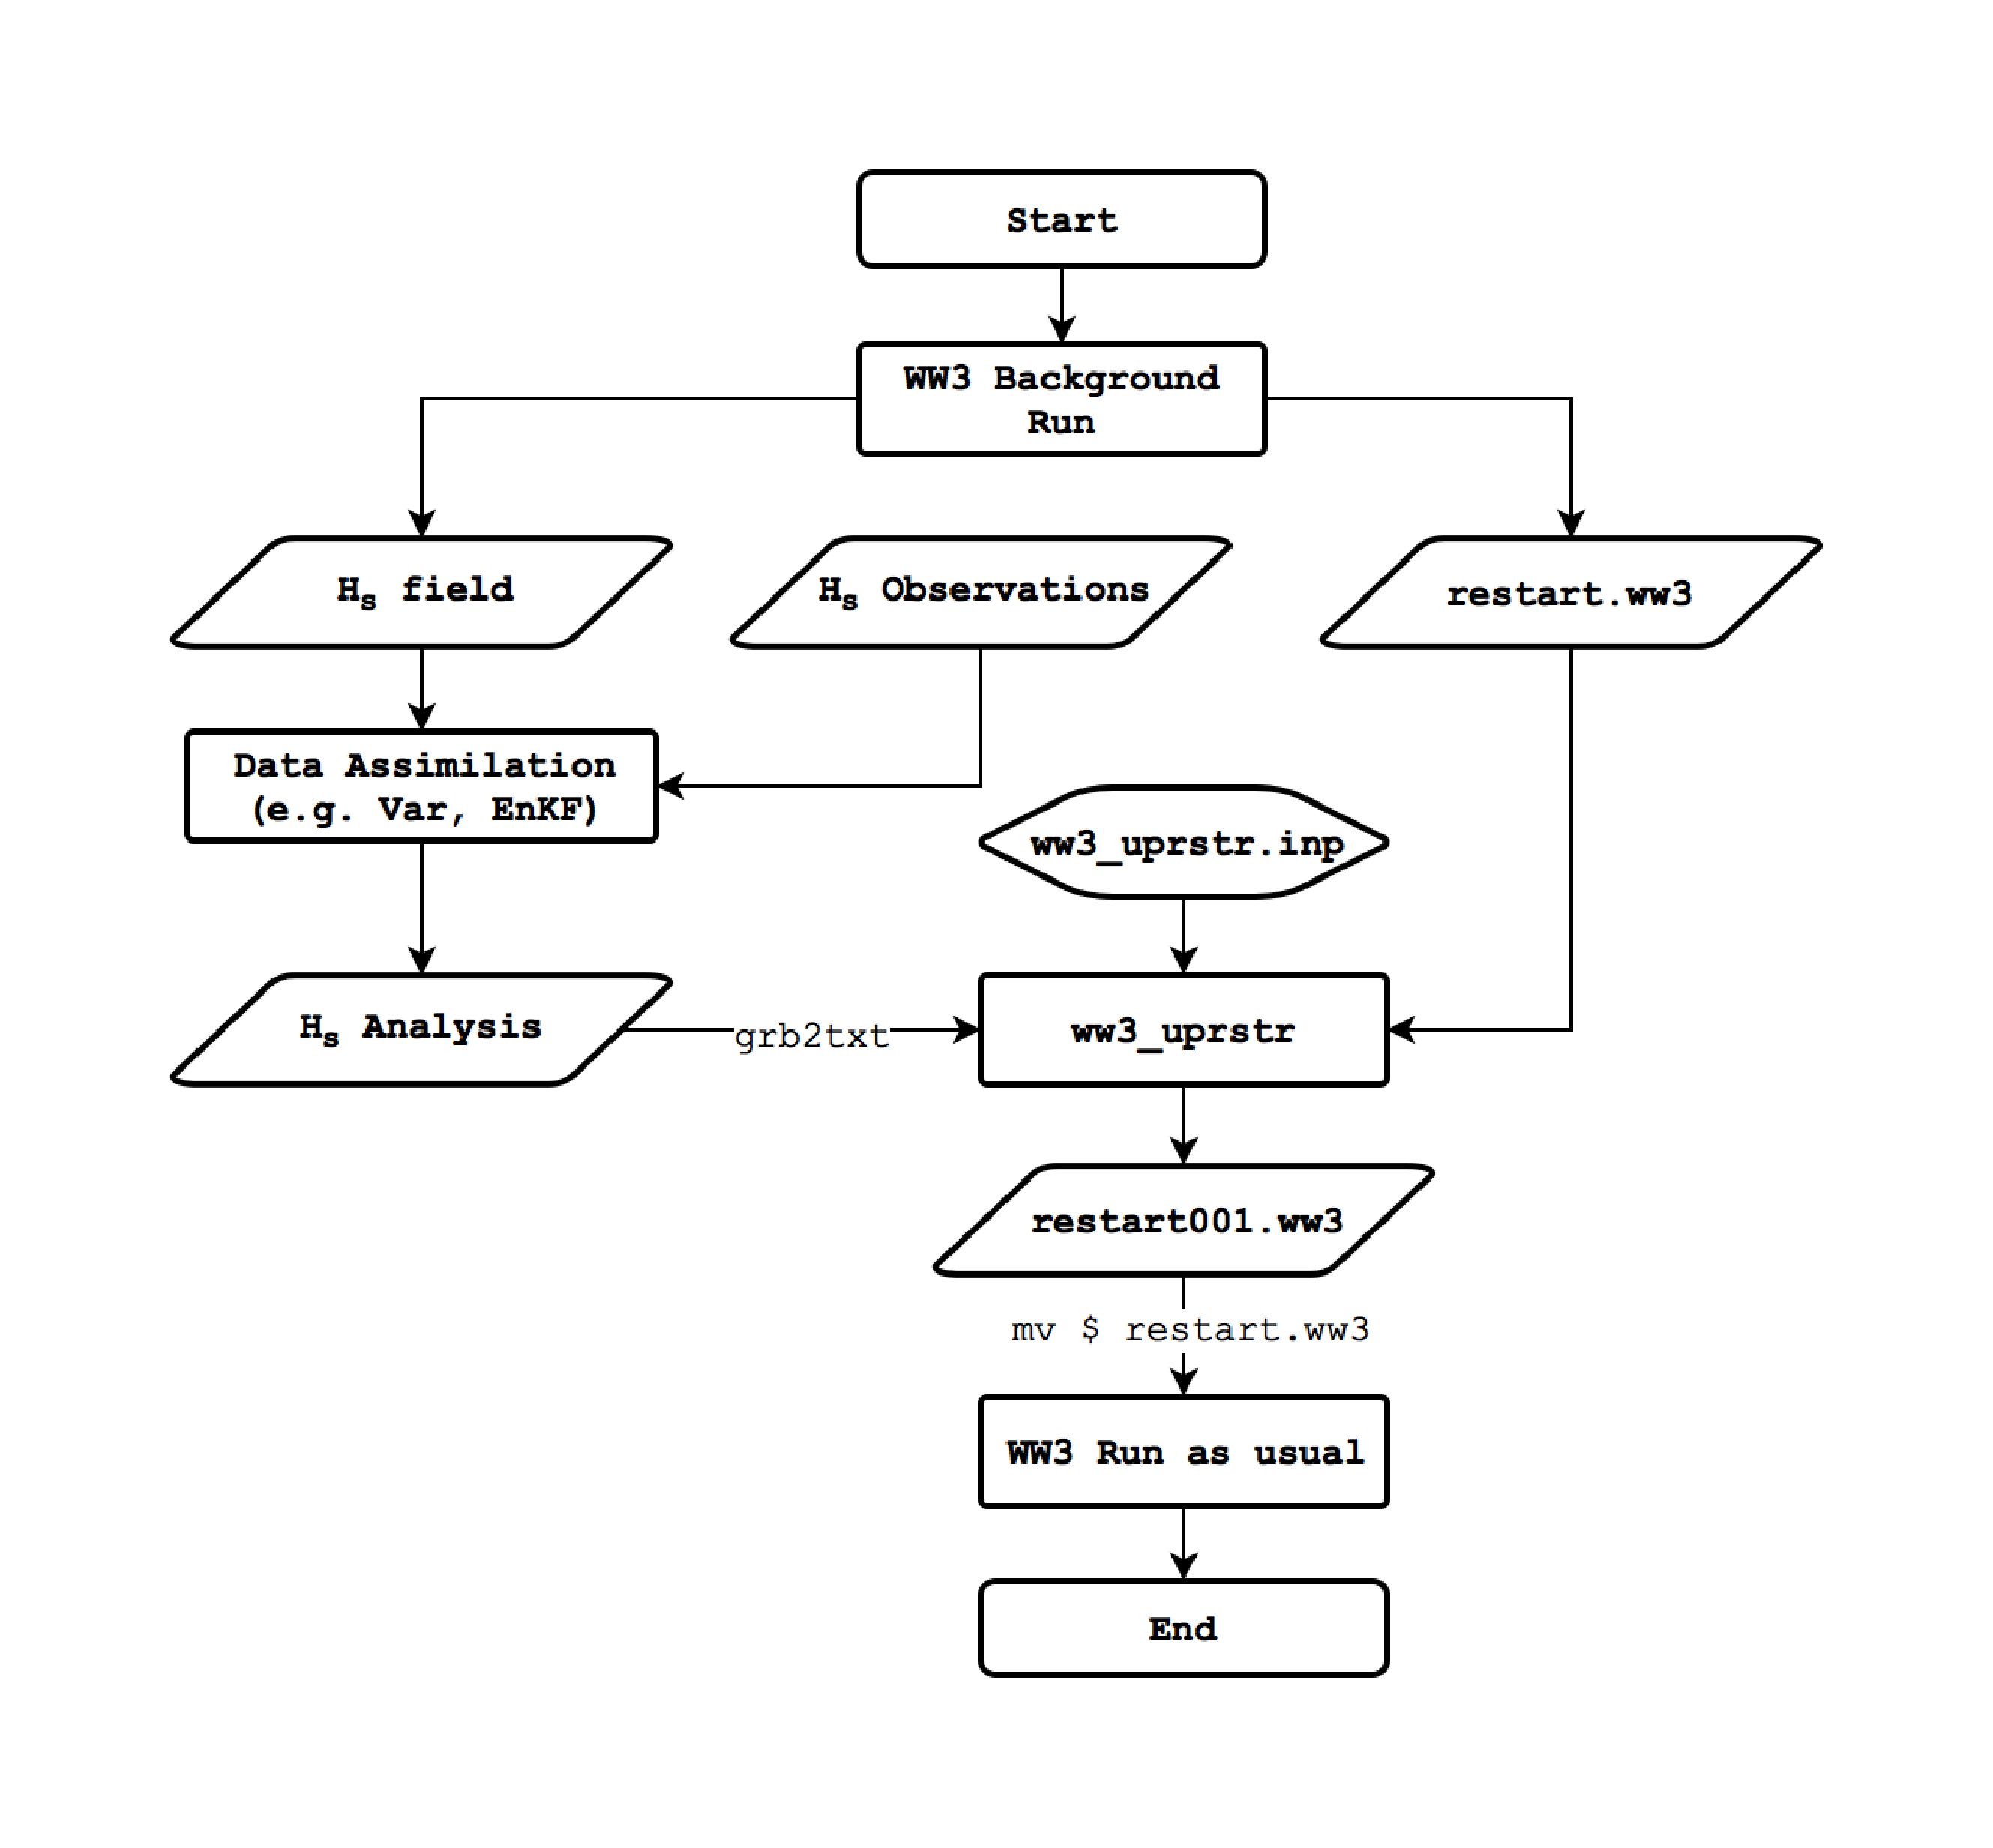
\includegraphics[width=0.9\textwidth]{./run/waveDA.eps}
\caption{简化波浪资料同化系统的流程图，展示 {ww3\_uprstr} 的作用、所需输入文件以及更新后重启动文件的输出结果。}
\label{fig:waveDAflowchart} \botline
\end{center}
\end{figure}

WDA 模块使用背景场和分析时刻可用的观测，生成分析，并以 grbtxt 格式（\textbf{XXXX.grbtxt}）导出 SWH 场。

分析文件、\textbf{mod\_def.ww3}、\textbf{restart.ww3} 文件以及 \textbf{ww3\_uprstr.inp} 是 \textbf{ww3\_uprstr} 的输入文件。如果所有选项和输入文件都准备正确，在单处理器上更新包含 260000 个网格节点的网格并生成输出大约需要一分钟。更新后的重启动文件必须改名为预期文件名；在本例中为 \textbf{restart.ww3}。\newline

   \noindent\fbox{
      \parbox{\textwidth}{
      \textbf{注意：}
      所有 \ncep{} 的 WDA 系统都使用 GRIB2 格式，因此总是需要一个中间步骤将 grib 文件转换为合适格式。所用软件为 WGRIB2，更多信息可从
      \href{http://www.cpc.ncep.noaa.gov/products/wesley/wgrib2}{官方网站} 获取。
      }
   }

%\paragraph{如何更新 ww3\_uprstr \newline}
%添加数据读取器，主要用于机器无关二进制数据和 wgrib2。

\pb


% tab:fields

\begin{table} \begin{center}
\begin{tabular}{|c|c|c|c|c|c|} \hline
组 & 字段 & 说明                  &  文件        & GRIB1 & GRIB2   \\
      &                              &  扩展名   & 数据  & 数据    \\ \hline \hline
 1 & 1 & 水深                           & {\file .dpt} &  --  &    --    \\
 1 & 2 & 平均海流分量         & {\file .cur} &  --  &    --    \\
 1 & 3 & 风速                      & {\file .wnd} &  32  &  0,2,1   \\
   &&  风向                 &              &  31  &  0,2,0   \\
   &&  风 $u$                       &              &  33  &  0,2,2   \\
   &&  风 $v$                       &              &  34  &  0,2,3   \\
 1 & 4 & 气海温差              & {\file .dt}  &  --  &    --    \\
 1 & 5 & 水位                     & {\file .wlv} &  --  &  10,3,1  \\
 1 & 6 & 海冰覆盖率                    & {\file .ice} &  91  &  10,2,0  \\
 2 & 1 & 波高 $H_s$               & {\file .hs}  & 100  &  10,0,3  \\
 2 & 2 & 平均波长                & {\file .l}   &  --  &    --    \\
 2 & 3 & 平均波周期 $T_{m0,2}$     & {\file .t02} &  --  &    --    \\
 2 & 4 & 平均波周期 $T_{m0,1}$     & {\file .t}   & 103  &  10,0,15 \\
 2 & 5 & 平均波周期 $T_{m0,-1}$    & {\file .tm1} &  --  &    --    \\
 2 & 6 & 峰值频率 $f_p$            & {\file .fp}  & 108  &  10,0,11 \\
 2 & 7 & 平均波向 $\theta_m$  & {\file .dir} & 101  &    --    \\
 2 & 8 & 方向扩展 $\sigma$     & {\file .spr} &  --  &    --    \\
 2 & 9 & 峰值方向 $\theta_p$       & {\file .dp}  & 107  &  10,0,10 \\
 4 & 1 & 分区 $H_s$              & {\file .phs} & 102,105 & 10,0,5/8 \\
 4 & 2 & 分区 $T_p$              & {\file .ptp} & 110,106 & 10,0,6/9\\
 4 & 3 & 分区 $L_p$              & {\file .plp} &  --  &    --    \\
 4 & 4 & 分区 $\theta_m$         & {\file .pdir} & 109,104 & 10,0,4/7 \\
 4 & 5 & 分区 $\sigma$           & {\file .psi} &  --  &    --    \\
 4 & 6 & 分区风海比例      & {\file .pws} &  --  &    --    \\
 4 & 7 & 总风海比例         & {\file .wsf} &  --  &    --    \\
 4 & 8 & 分区数            & {\file .pnr} &  --  &    --    \\
 5 & 1 & 摩擦速度分量         & {\file .ust} &  --  &    --    \\
 5 & 2 & 空气侧 Charnock 参数 & {\file .cha} &  --  &    --    \\
 5 & 3 & 能量通量 $\int C_g E(f) df$  & {\file .CgE} &  --  &    --    \\
 5 & 4 & 风到波能量通量        & {\file .faw} &  --  &    --    \\
 5 & 5 & 波支撑应力           & {\file .taw} &  --  &    --    \\
 5 & 6 & 向上波支撑应力    & {\file .twa} &  --  &    --    \\
 5 & 7 & 白冠覆盖率              & {\file .wcc} &  --  &    --    \\
 5 & 8 & 平均白冠泡沫厚度 & {\file .wcf} &  --  &    --    \\
 5 & 9 & 有效破碎波高& {\file .wch} &  --  &    --    \\
 5 & 10 & 白冠矩                 & {\file .wcm} &  --  &    --    \\ \hline
\end{tabular} \end{center}
\caption{~场输出后处理器辅助数据。} \label{tab:fields}
\vspace{0.5in}
\end{table}

\begin{table} \begin{center}
\begin{tabular}{|c|c|c|c|c|c|} \hline
组 & 字段 & 说明                  &  文件        & GRIB1 & GRIB2   \\
      &                              &  扩展名   & 数据  & 数据    \\ \hline \hline
 6 & 1 & 辐射应力                & {\file .Sxy} &  --  &    --    \\
 6 & 2 & 破碎波动量通量     & {\file .two} &  --  &    --    \\
 6 & 3 & Bernoulli 水头                  & {\file .J} &  --  &    --    \\
 6 & 4 & 破碎波能量通量       & {\file .foc} &  --  &    --    \\
 6 & 5 & Stokes 输运                & {\file .tus} &  --  &    --    \\
 6 & 6 & 表层 Stokes 漂移            & {\file .uss} &  --  &    --    \\
 6 & 7 & $k=0$ 处二阶压力  & {\file .p2s} &  --  &    --    \\
 7 & 1 & 近底振幅           & {\file .cfd} &  --  &    --    \\
 7 & 2 & 近底速度            & {\file .ubr} &  --  &    --    \\
 7 & 3 & 床形参数              & {\file .bed} &  --  &    --    \\
 7 & 4 & 到底部边界层的能量通量 & {\file .fbb} &  --  &    --    \\
 7 & 5 & 到底部边界层的动量通量 & {\file .tbb} &  --  &    --    \\
 8 & 1& 平均平方坡度              & {\file .mss} &  --  &    --    \\
 8 & 2 & Phillips 常数               & {\file .msc} &  --  &    --    \\
 9 & 1 & 平均时间步长               & {\file .dtd} &  --  &    --    \\
 9 & 2 & 截止频率 $f_c$         & {\file .fc}  &  --  &    --    \\
 9 & 3 & 截止频率 $f_c$         & {\file .fc}  &  --  &    --    \\
 9 & 4 & X-Y 平流最大 CFL   & {\file .cfx} &  --  &    --    \\
 9 & 5 & $\theta$ 平流最大 CFL & {\file .cfd} &  --  &    --    \\
 9 & 6 & $k$ 平流最大 CFL   & {\file .cfk} &  --  &    --    \\
 10 & 1 & 用户定义 \#1                & {\file .us1} &  --  &    --    \\
 10 & 2 & 用户定义 \#2                & {\file .us2} &  --  &    --    \\ \hline
\end{tabular} \end{center}
\caption*{表~\ref{tab:fields}，续。}
\vspace{0.5in}
\end{table}

\clearpage
